%==========================オプションおよび文書クラスの設定==========================
%"autodetect-engine"-どのエンジンでもコンパイル可能にするオプション
%"dvipdfmx-if-dvi"-必要な場合のみdvipdfmx経由のpdf化をするオプション(LuaTeXやXeTeXはPDFに直接変換するため)
%"ja=standard"-日本語文書の標準設定を利用するオプション
%"bxjs…"-どのエンジンでも利用可能なドキュメントクラス
%--以下のいずれかを選択--
\documentclass[autodetect-engine,dvipdfmx-if-dvi,ja=standard,a4paper,11pt]{bxjsarticle} %章の無いレポート
%\documentclass[autodetect-engine,dvipdfmx-if-dvi,ja=standard,a4paper,10pt]{bxjsslide} %スライド
%\documentclass[autodetect-engine,dvipdfmx-if-dvi,ja=standard,a4paper,10pt]{bxjsbook} %書籍
%\documentclass[autodetect-engine,dvipdfmx-if-dvi,ja=standard,a4paper,10pt]{bxjsreport} %章のある論文やレポート

%==============================プリアンブルの設定==============================
\title{春期課題} %タイトル
\author{新B4 福田真悟} %著者名
\date{2020.3.3}%日付 %日付下の余白をN[mm]減らす

%///////////////////////////////////////////////////////////////////////////////////////////////////////////
%////////////////////////////////////パッケージの読込み及び設定の書換え//////////////////////////////////////
%///////////////////////////////////////////////////////////////////////////////////////////////////////////
\usepackage{graphicx} %図の挿入に関するパッケージ
\usepackage{float} %[H]で図の位置を固定する機能をONにするパッケージ
\usepackage{subcaption} %サブキャプションに関するパッケージ
\captionsetup{labelsep=space} %サブキャプション後の":"を非表示にする
\usepackage{enumerate} %{enumerate}[]の,[]の中の通りの箇条書きにすることができるパッケージ
\usepackage{amsmath} %数式に関するパッケージ
\usepackage{mathtools} %数式に関するパッケージ
\usepackage{bm} %ベクトル表示のコマンドを追加するパッケージ
\usepackage{comment} %複数行のコメントアウトを可能にするパッケージ
\usepackage{ascmac} %枠に関するパッケージ
\usepackage{tabularx} %表に関するパッケージ
\setpagelayout{top=10truemm,bottom=15truemm,left=15truemm,right=15truemm}  %余白に関する設定の書換え(bxjs…クラスではgeometryパッケージは使用不可)
\graphicspath{{../figures/}} %図を挿入する際に.texファイルの上の階層にあるfiguresというフォルダを参照可能にする
\usepackage{url}

%余白に関する設定の書換え(bxjs…クラスではgeometryパッケージは使用不可)
\belowcaptionskip=-0pt %キャプション下の余白をN[pt]減らす
\graphicspath{{../figures/}} %図を挿入する際に.texファイルの上の階層にあるfiguresというフォルダを参照可能にする

%使用記号の追加
\newcommand{\divergence}{\mathrm{div}\,}  %ダイバー
\newcommand{\grad}{\mathrm{grad}\,}  %グラディエント
\newcommand{\rot}{\mathrm{rot}\,}  %ローテーション

%\pagestyle{myheadings} %myheading文字列 emptyページ番号なし plainフッダーに
%\markright{\footnotesize 2月28日(金)15:00~ 顔合わせ}%全ページ共通への挿入
%================================以下本文================================
\begin{document}
\maketitle %設定したタイトルの挿入
\section{\normalsize"Lorenz 方程式","Rossler 方程式","ホワイトガウスノイズ","Logistic 写像"
,"順列エントロピー","相互情報量","複雑ネットワーク"について書籍やインターネットで調べる
}%sectionの前に*をつけると数字の振り分けが消える不思議


\begin{figure}[H]%[h]は記述したところ。[t]はそのページの上端。[t]はそのページの下端、[p]はページいっぱい
\begin{center}
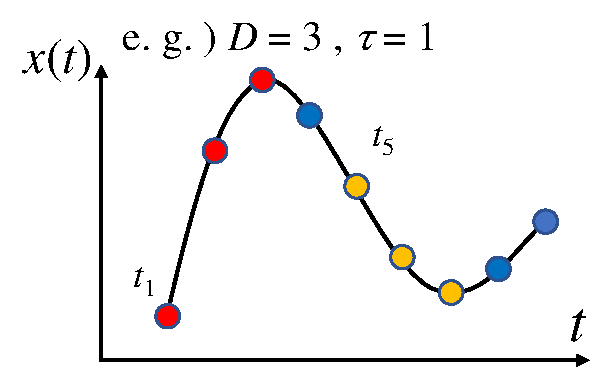
\includegraphics[width=.4\textwidth]{crop_PE1ver2.pdf} 
\end{center}
\caption{時系列$ x(t) $}%図名
\label{PE1}
\end{figure}


\begin{itemize}
\item Lorenz 方程式\\
非線形な微分方程式の1つで
\begin{equation}
\csc \theta = \frac{1}{\sin \theta}
\end{equation}

\item Rossler 方程式\\

\item ホワイトガウスノイズ\\

\item Logistic 写像\\

\item 順列エントロピー\\

\item 相互情報量\\

\item 複雑ネットワーク\\

\end{itemize}


\section{\normalsize相互情報量とLorenz 方程式に関するMATLAB ファイル(mutual.m) を実行し,図を出力する}



\section{\normalsizeホワイトガウスノイズと順列エントロピーに関するMATLABファイル(B4kadai\_2020.m)を実行し,図を出力し考察を加える.}



%$A^1$\cite{aaa}%参考文献




%\begin{itemize}
%\item アイテムコード1
%\item アイテムコード2
%\item アイテムコード3
%\item アイテムコード4
%\item アイテムコード5
%\end{itemize}

%\begin{itemize}
%\item Lorenz 方程式\\
%非線形な微分方程式の1つで
%\begin{equation}
%\csc \theta = \frac{1}{\sin \theta}
%\end{equation}



\begin{thebibliography}{9999}%参考文献
\bibitem{aaa}%参考文献citeするぞ
後藤田研究室HP,\url{https://www.rs.tus.ac.jp/gotodalab/index.html}
\bibitem{Latex}
簡単LaTeXインストールWindows編(2016年4月版),\url{https://did2memo.net/2016/04/24/easy-latex-install-windows-10-2016-04/}
\end{thebibliography}

%\newpage



\end{document}